% sudo apt install texlive-latex-base texlive-lang-cyrillic texlive-latex-recommended texlive-latex-extra
% pdflatex Polyarniy_CV.pdf

\documentclass[11pt,oneside]{article}
\usepackage[utf8]{inputenc}
\usepackage[english,russian]{babel}
\usepackage{xcolor}
\usepackage{hyperref}
\usepackage[left=3cm,right=3cm,top=3cm,bottom=3cm]{geometry}

\usepackage{graphicx}
\usepackage{wrapfig}
\usepackage[absolute,overlay]{textpos}
\graphicspath{ {imgs/} }

\newcommand{\hhref}[2]{\href{#1}{\color{blue}#2}}

\begin{document}

\begin{textblock}{7}(9,0.42)
    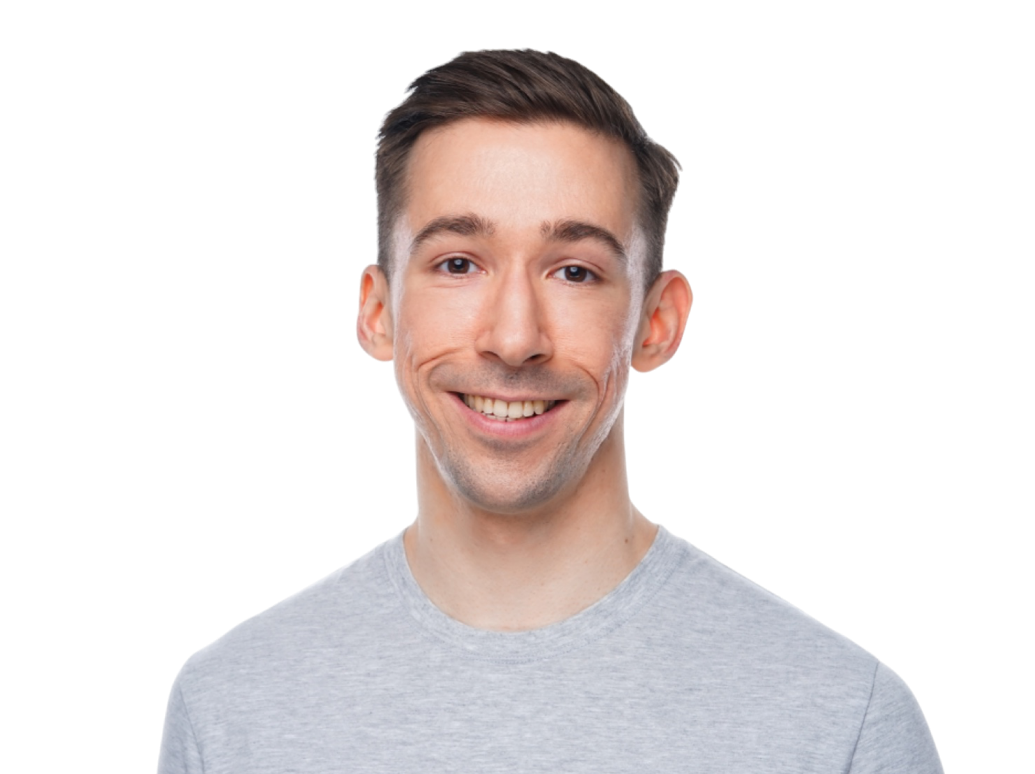
\includegraphics[scale=0.6]{photo2025.png}
\end{textblock}

\begin{center}
	{\huge Poliarnyi Nikolai \\ Полярный Николай}
\end{center}

\vspace{-9pt}
\section*{\textbf{Work Experience}}
\vspace{-9pt}


\begin{description}
  \item[ - \hhref{https://en.wikipedia.org/wiki/PhotoScan}{Agisoft Metashape}] \hfill \\
    \textbf{Since April 2016}

    \textbf{Mathematician-Programmer (Team Lead)}

    R\&D: tune performance, pioneer innovations, identify\&eliminate major user pain points.

    \begin{itemize}

      \item Invented a scalable, multi-scale surface reconstruction method (out-of-core/cluster-friendly), \hhref{https://www.polarnick.com/static/papers/poliarnyi2021.pdf}{published a paper} at \hhref{http://iccv2021.thecvf.com/}{ICCV 2021}.
      \item Developed GPU-accelerated algorithms (using custom OpenCL/CUDA/Vulkan wrappers), including: depth maps reconstruction and out-of-core texture generation.
      \item Enhanced cloud performance, achieving 2x faster processing.
      \item Photographed (15K images) and digitized the UNESCO site \hhref{https://heritage3d.ru/models/kizhskiy-pogost}{Kizhi Pogost}.
      \item Set up in-office local LLM server.
    \end{itemize}

    Computer Vision, Computational Geometry, OpenCL/CUDA/Vulkan, \hhref{https://polarnick.com/static/presentations/AgisoftMetashapeGSW2023.pdf}{LiDAR}, AI/ML
  \item[ - Transas] \hfill \\
    \textbf{October 2014 - March 2016}

    \textbf{Mathematician-Programmer}

    Developed a server that produces 3D landscape reconstruction and true orthophoto stitching from UAVs' data.
    % (\hhref{http://polarnick239.github.io/old/cv/Monoceros1.pdf}{presentation}, \hhref{http://polarnick239.github.io/old/cv/Monoceros2.pdf}{second presentation}).

    OpenCV, OpenCL, Python, Cython, Ceres-solver
  \item[ - Yandex.Money] \hfill \\
    \textbf{February 2014 – October 2014:} Software Developer (Java backend)
  \item[ - DevExperts] \hfill \\
    \textbf{April 2013 – September 2013:} Software Developer (Java backend)

\end{description}


\vspace{-9pt}
\section*{\textbf{Skills}}
\vspace{-9pt}

\begin{itemize}
    \item{\textbf{Computer Vision}}: Structure from Motion, Multiple View Geometry, AI/ML, objects detection/classification/segmentation, magic.
    Better than state of the art depth maps estimation, surface reconstruction, texturing and other algorithms.

    \item{\textbf{Computational geometry, CGAL}}: computations with absolute accuracy, algorithms and structures like Delaunay triangulation.

    \item{\textbf{\hhref{https://github.com/GPGPUCourse/GPGPUVulkan}{Vulkan}, OpenCL, CUDA, OpenGL, WebGL}}: GPGPU computations, shaders, ray tracing, algorithms profiling/acceleration/adaptation for the GPU. Able to work around bugs in video drivers and compilers.

    \item{\textbf{C++, Python, Java}}
\end{itemize}


\vspace{-9pt}
\section*{\textbf{Activities}}
\vspace{-9pt}

\begin{itemize}
    \item{\textbf{Consultant}}: provides consultation/project-development services to companies and startups on topics related to Computer Vision and GPU-acceleration.

    \item{\textbf{Public lectures}}: \hhref{https://csspace.io/open-lecture/2025-gpu}{GPGPU in CS Space}, \hhref{https://www.youtube.com/watch?v=adQQoH3iXPQ}{Science Day in school}, \hhref{https://www.youtube.com/watch?v=ltUzX1IR9JI&list=PL5p-5hHpsHBolSeDn7__1c9hgPprYTjnn&index=3}{Algorithms behind Unreal Engine 5 Nanite tech}.

    \item{\textbf{Photogrammetry course}}: developed Photogrammetry  \hhref{https://compsciclub.ru/courses/photogrammetry/2021-spring/}{course} in Computer Science Club. Teaching it in \hhref{https://math-cs.spbu.ru/}{SPbU} and \hhref{https://ct.itmo.ru/}{ITMO}.  \hhref{https://www.youtube.com/watch?v=rEF0zkv2cn8&list=PL5p-5hHpsHBp4yTpeZJ_QMSmJPAuov-VF&index=1}{Video recordings}. Tasks on \hhref{https://github.com/PhotogrammetryCourse/}{github}.

    \item{\textbf{GPGPU course}}: developed GPGPU OpenCL \hhref{https://compscicenter.ru/courses/video_cards_computation/}{course} in Computer Science Center. \hhref{https://www.youtube.com/watch?v=LDt4KQEdImY&list=PLlb7e2G7aSpSkDWlyJQzT9Qx9rrgKSgAp&index=1}{Video recordings}. Tasks on \hhref{https://github.com/GPGPUCourse/}{github}.

    \item{\textbf{Open-source}: \hhref{https://github.com/GPGPUCourse/GPGPUVulkan}{Vulkan API library}. \hhref{https://github.com/PolarNick239/ExternalSortingOnGPU}{Out-of-core merge sort} with GPU acceleration. \hhref{https://gist.github.com/PolarNick239/7819fb7722fab09b37ecaee77c82cf58}{96-bit 3D Morton code}. OpenCL \hhref{https://github.com/PolarNick239/OpenMeanShift}{implementation} of EDISON mean shift. \hhref{https://github.com/opencv/opencv/pull/6078}{Implemented} Python bindings for OpenCL algorithms in OpenCV. Contributions to OpenCV, PyOpenCL, jupyter qtconsole and others. GPU monitoring in i3pystatus.}

    \item{\textbf{Hackathons}}: six awards on hackatons. Two first places on \hhref{https://github.com/PolarNick239/HackathonDroneSwarm}{X-Mas Hack} (mission planner for drone swarm). Third place on \hhref{https://career.luxoft.com/lp/hack-cv/}{HackCV} (traffic signs recognition), \hhref{http://hackday.ru/sciencehackday-2/projects\#project-1400}{Science Hackday \#2} (Startup nomination), \hhref{http://hackday.ru/hackday-36/projects\#project-1121}{Hackday\#36} (Autodesk 3D-web nomination), \hhref{https://www.hackerleague.org/hackathons/jetbrains-edtech-hackathon/blogposts/53655896e24d32cfbd000006}{HackEdu} by JetBrains (third place). Participation in \hhref{http://www.hackjunction.com/}{Junction 2016, 2017}.

    \item{\textbf{Conferences}}: published \hhref{https://www.polarnick.com/static/papers/poliarnyi2021.pdf}{a paper} on \hhref{http://iccv2021.thecvf.com/}{ICCV 2021}. Presented the report \hhref{https://polarnick.com/static/presentations/AgisoftMetashapeGSW2023.pdf}{LiDAR and Photogrammetry Compared and Combined} at the \hhref{https://gsw2023.com/}{ISPRS GSW 2023 Conference}. Participated in \hhref{http://3dv18.uniud.it/}{3DV 2018} and \hhref{http://www.3d-arch.org/}{3D-ARCH 2019}.

    \item{\textbf{Magister Ludi}}: \hhref{http://239.ru}{PML №239} programming teacher. Supervising 20+ student game dev projects \hhref{https://www.youtube.com/watch?v=bbKXnsysUXw}{each year}.
\end{itemize}

\vspace{-9pt}
\section*{\textbf{Education}}
\vspace{-9pt}

\begin{itemize}
    \item{Computer Science Center}
    \item{ITMO University, Computer Technologies}
    \item{PML №239, mathematical circle, programming contests}
\end{itemize}

\begin{wrapfigure}{r}{0.22\textwidth}
    \centering
    \includegraphics[width=0.22\textwidth]{unicorn.png}
\end{wrapfigure}

\vspace{-9pt}
\section*{\textbf{Contacts}}
\vspace{-9pt}

\begin{itemize}

    \item{\textbf{\hhref{mailto:PolarNick239@gmail.com}{PolarNick239@gmail.com}}}

    \item{\textbf{\hhref{http://polarnick239.github.io/index_ru.html}{PolarNick.ru}}}

    \item{\textbf{\hhref{https://github.com/PolarNick239}{GitHub}}}

    \item{\textbf{\hhref{https://www.linkedin.com/in/nikolai-poliarnyi-61393b7b}{LinkedIn}}}

\end{itemize}

Last updated: 15.05.2025

\end{document}
